\chapter{Machinery}\label{chap:machinery}
\setlength\epigraphwidth{.85\textwidth}
\epigraph{``Now stop!'' Max said and sent the wild things off to bed\\
  without their supper. And Max the king of all wild things was lonely\\
  and wanted to be where someone loved him best of all.}{---Maurice
  Sendak, \emph{Where the Wild Things Are}}

In this chapter, we develop two pieces of machinery that are extremely
useful in working with general topological ambient isotopies. The
first is a \emph{uniform convergence} version of
\cref{thm:countable-gluing-ambient-isotopies}, which has the benefit
of not requiring disjointness for our $V_n$. This is a double-edged
sword: On the one hand, it affords us greater latitude in the kinds of
situations where we can apply it, but on the other, it is much easier
to accidentally misuse.

The second is \emph{separation of strands}, which essentially allows
us to partition our knot into segments that are all ``isolated'' from
each other except at their ends (where they share mutual points with
the neighboring strands).\footnote{Note, we will not make any
  guarantees about how complicated the segments themselves look, only
  that they are separated from each other.} This will allow us to work
``locally'' on our knots by keeping our ambient isotopies contained to
regions where they can only affect one part, which will prove
indispensable in the subsequent chapters.




\section{Uniform Convergence and Ambient Isotopy}
% The next theorems will form the backbone of more-or-less all of our
% examination of general topological embeddings.
The following theorems will play a central role in allowing us to
prove all arcs are ambient isotopic in $\RR^2$. The idea is to use
uniform convergence to concatenate countably-many ambient isotopies
together without breaking any of our continuity concerns. We first
recall some definitions from Analysis, then we prove the ambient
isotopy uniform convergence theorem.
\begin{definition}[Uniform Convergence]
  Let $(E,d)$, $(E', d')$ be metric spaces, and for all $n \in \NN$,
  let $f_n : E \to E'$. Also let $f : E \to E'$. Then we say $f_n \to
  f$ \emph{uniformly} iff for all $\varepsilon > 0$, there exists $N
  \in \NN$ such that if $n > N$, then $\forall x \in E$,
  \[
    \abs{f(x) - f_n(x)} < \varepsilon.
  \]
  We will sometimes denote uniform convergence by $f_n \xrightarrow{u}
  f$.
\end{definition}
\begin{proposition}\label{prop:uniform-convergence}
  For all $n \in \NN$, let $f_n : E \to E'$ be a continuous function.
  Now, let $f : E \to E'$, and suppose that $f_n \uconv f$. Then $f$
  is continuous.
\end{proposition}
The proof is an $\frac{\varepsilon}{3}$ argument and can be found in
any standard analysis text.
                        %                         \begin{corollary}
                        %                         Let $E, E', E''$ be compact metric spaces. For all $n \in \NN$, let
                        %                         $f_n : E \to E'$ and $g_n : E' \to E''$ be continuous. Also let $f:
                        %                         E \to E'$ and $g : E' \to E''$, and suppose that $f_n \uconv f$ and
                        %                         $g_n \uconv g$. Then for all $x \in E$,
                        %                         \[
                        %                         \lim_{n\to\infty} (g_n \circ f_n)(x) = (g \circ f)(x).
                        %                         \]
                        %                         \end{corollary}
                        %                         \begin{sproof}
                        %                         Let $\varepsilno$
                        %                         \end{sproof}

\begin{corollary}\label{cor:uniformly-convergent-homeomorphisms}
  Let $(E, d)$, $(E', d')$ be metric spaces, and for all $n \in \NN$,
  let $f_n : E \to E'$ such that $f_n$ is a homeomorphism. Let $f : E
  \to E'$ be a bijection and suppose that
  \begin{enumerate}
    \item $f_n \uconv f$, and
    \item $f^{-1}_n \uconv f^{-1}$
  \end{enumerate}
  Then $f$ is a homeomorphism.
\end{corollary}
\begin{sproof}
  Continuity of $f$, $f^{-1}$ follows directly from
  \cref{prop:uniform-convergence}. Bijectivity gives us a
  homeomorphism.
\end{sproof}

% \begin{question}
%   Is it possible to drop one of (a) bijectivity, or (b) $f_{n}^{-1}
%   \uconv f^{-1}$? In all of the examples we have found where one
%   breaks, the other breaks too. It seems that there should be a
%   straightforward proof using
% \end{question}

% \begin{proposition}
%   Let $f_n : E \to E'$ such that $f_n$ is a homeomorphims. Let $f : E
%   \to E'$ be a bijection, and suppose that $f_n \uconv f$. Then
%   $f_n^{-1} \uconv f^{-1}$.
% \end{proposition}
% \begin{proof}
%   Let $\varepsilon > 0$ be given. Then there exists $N \in \NN$ such
%   that $n > N$ implies that for all $x \in E$, $f_n(x) \in
%   B_\varepsilon(f(x))$.
% \end{proof}
% \begin{sproof}

% \end{sproof}


% \begin{question}
%   Is it possible to drop the bijectivity requirement here, in light of
%   both $f_n \uconv f$ and $f_n^{-1} \uconv f^{-1}$?
% \end{question}
% \begin{remark}
%   It is not possible to drop the bijectivity condition. We'll see an
%   example of why in \cref{ex:fox-artin-curve}.
% \end{remark}


% \subsection{Uniform Convergence and Ambient Isotopy}
We have the following straightforward lemma.
\begin{lemma}\label{lem:countable-homeomorphisms}
  Let $(E,d)$ be a metric space. For all $k\in\NN$, let $V_k \subseteq
  E$, and let $f_k : E \to E$ be a homeomorphism such that $f_k$ is
  identity on $E \setminus V_k$. Define $f : E \to E$ by
  \begin{align*}
    f
    &= \lim_{n\to\infty} \comp_{k=1}^n f_k \\
    &= \lim_{n\to\infty} \pn{f_n \circ f_{n-1} \circ \cdots \circ
      f_{2} \circ f_1}.
  \end{align*}
  Then provided
  \begin{enumerate}
    \item $f$ is a bijection,
    \item The $g^{-1}_n$ defined by $g_n^{-1} = f_1^{-1} \circ \cdots
      \circ f_{n-1}^{-1} \circ f_n^{-1}$, satisfy $g_n^{-1} \uconv
      f^{-1}$, and
    \item The $V_k$ satisfy
      \[
      \lim_{n\to\infty} \mrm{diam}\pn{\bigcup_{k=n}^\infty V_k} = 0,
      \]
  \end{enumerate}
  Then $f$ is a homeomorphism.
\end{lemma}
\begin{remark}
  Note, if $E$ is a compact Hausdorff space, we can drop the condition
  on the $g_n^{-1}$'s, since a continuous bijection from a compact
  space to a Hausdorff space is always a homeomorphism. In particular,
  if $\bigcup_{k=1}^\infty V_k$ is bounded in some compact set, then
  it suffices to prove $f$ is continuous. We stated the more general
  version of the result here, but from now on, we will generally
  assume that we have this simplifying condition.
\end{remark}
\begin{sproof}
  For all $n\in \NN$, define
  \[
    g_n = \comp_{k=1}^n f_k,
  \]
  and note that it is a homeomorphism with inverse
  \begin{align*}
    g^{-1}_n
    &= \comp_{k=1}^n f^{-1}_{n+1-k} \\
    &= f^{-1}_{1} \circ f^{-1}_2 \circ \cdots \circ f^{-1}_{n-1} \circ
      f^{-1}_n.
  \end{align*}
  Since we assume bijectivity of $f$ and $g_n^{-1} \to f^{-1}$ (thus
  $f^{-1}$ is continuous) by hypothesis, it suffices to show that $f$
  is continuous. To that end, we want to show $g_n \uconv f$. Let
  $\varepsilon > 0$ be given. Note that because
  \[
    \lim_{n\to\infty} \mrm{diam}\pn{\bigcup_{k=n}^\infty V_k} = 0,
  \]
  there exists $n_0 \in \NN$ such that $n > n_0$ implies
  \[
    \mrm{diam}\pn{\bigcup_{k=n}^\infty V_k} < \varepsilon.
  \]
  Hence, let $n > n_0$ be fixed, and let $U_n$ denote
  \[
    U_n = \bigcup_{k = n}^\infty V_k
  \]
  Observe that by definition, $f = g_n$ on $E \setminus U_n$, hence
  they are trivially $\varepsilon$-close on $E \setminus U_n$.

  For showing $\varepsilon$-closeness on the $U_n$, note that
  $\fim{f}{U_n} = \fim{g_n}{U_n}$. Thus because $\mrm{diam}(U_n) <
  \varepsilon$, it follows that $f, g_n$ are $\varepsilon$-close on
  $U_n$ as well. Hence $g_n \uconv f$, so $f$ is continuous.

  By \cref{cor:uniformly-convergent-homeomorphisms}, it follows that
  $f$ is a homeomorphism.
\end{sproof}




This extends naturally to the following version for ambient isotopies.
The statement might appear a bit complicated, but it's really just
saying that whenever we're given a collection of ambient isotopies
that are restricted to acting on sets whose radii decay sufficiently
quickly, we can play countably many of them back-to-back in finite
time and yield an ambient isotopy.
\begin{theorem}[Ambient Isotopy and Uniform
  Convergence]\label{thm:uniformly-convergent-ambient-isotopy}
  Let $(E,d)$ be a metric space. For all $k \in \NN$, let $V_k
  \subseteq E$, and let $F_k : [0,1] \times E \to E$ be an ambient
  isotopy such that $F_k$ is identity on $[0,1] \times (E \setminus
  V_k)$. For all such $k$, define $f_k(x) : E \to E$ by $f_k(x) =
  F_k(1, x)$; note that by definition of ambient isotopy, $f_k(x)$ is
  a homeomorphism. Then define $F : [0,1] \times E \to E$ as follows:
  For all $(t,x) \in [0,1] \times E$, let
  \[
    F(t, x) =
    \begin{cases}
      F_1(2t, x) & \text{if } t \in \bk{0, \frac{1}{2}} \\
      F_2(4 (t - 1/2), f_1(x)) & \text{if } t \in \pb{\frac{1}{2},
        \frac{3}{4}} \\
      F_3(8 (t - 3/4), f_2(f_1(x))) & \text{if } t \in
      \pb{\frac{3}{4}, \frac{7}{8}} \\
      \hspace{.5em} \vdots & \\
      F_n\pn{2^n \pn{t - 1 + \frac{1}{2^{n-1}}}, \comp_{k=1}^{n-1}
        f_k(x)} & \text{if } t \in \pb{1 - \frac{1}{2^{n-1}}, 1 -
        \frac{1}{2^n}} \\
      \hspace{.5em} \vdots & \\
      \comp_{k=1}^\infty f_k(x) & \text{if }t = 1.
    \end{cases}
  \]
  Then provided
  \begin{enumerate}
    \item $F(1, \cdot)$ is a bijection,
    \item $\bigcup_{k=1}^\infty V_k$ is bounded in a compact set, and
    \item The $V_k$ satisfy
      \[
      \lim_{n\to\infty} \mrm{diam}\pn{\bigcup_{k=n}^\infty  V_k} = 0,
      \]
  \end{enumerate}
  then $F$ is an ambient isotopy.
\end{theorem}
\begin{proof}
  Note that \np{$\bigcup_{k=1}^\infty V_k$ is bounded in a compact
    set} allows us to apply the simplifying condition for
  \cref{lem:countable-homeomorphisms}.
  \begin{enumerate}
    \item To show $F(0, \cdot)$ is identity: Observe $F(0, x) = F_1(0,
      x) = x$, since $F_1(0,x)$ is an ambient isotopy (and hence
      identity for $t=0$).
    \item To show $F(t, x)$ is a homeomorphism for each $t\in [0, 1)$:
      If $t \neq 1$, then there exists $n \in \NN$ such that $t \in
      \pb{1 - \frac{1}{2^{n-1}}, 1 = \frac{1}{2^n}}$. Hence
      \[
      F(t, x) = F_n\pn{2^n \pn{t - 1 + \frac{1}{2^{n-1}}},
      \comp_{k=1}^{n-1} f_k(x)},
      \]
      which is a finite composition of
      homeomorphisms, and thus a homeomorphism.\footnote{``Finite
      composition of homeomorphisms'' follows because for all $t' \in
      [0,1]$, $F_n(t', x)$ and $\comp_{k=1}^{n-1} f_k(x)$ are both
      homeomorphisms.}
    \item To show that $F(1, \cdot)$ is a homeomorphism: Observe that
      $F(1, \cdot)$ is a bijection, $f_k$ is constant on $E
      \setminus V_k$ for each $k$, and $\lim_{n\to\infty} \mrm{diam}
      \pn{\bigcup_{k=n}^\infty V_k} = 0$. Thus by
      \cref{lem:countable-homeomorphisms}, $F(1, \cdot)$ is a
      homeomorphism.
    \item Finally, to show that $F$ is continuous: Define a sequence
      of ambient isotopies $G_n : [0,1] \times E \to E$ such that
      \[
      G_n(t, x) =
      \begin{cases}
        F_1(2t, x) & \text{if } t \in \bk{0, \frac{1}{2}} \\
        F_2(4 (t - 1/2), f_1(x)) & \text{if } t \in \bk{\frac{1}{2},
          \frac{3}{4}} \\
        F_3(8 (t - 3/4), f_2(f_1(x))) & \text{if } t \in
        \bk{\frac{3}{4}, \frac{7}{8}} \\
        \hspace{.5em} \vdots & \\
        F_n\pn{2^n \pn{t - 1 + \frac{1}{2^{n-1}}}, \comp_{k=1}^{n-1}
          f_k(x)} & \text{if } t\in \bk{1 - \frac{1}{2^{n-1}}, 1 -
          \frac{1}{2^n}} \\
        \comp_{k=1}^n f_k(x) & \text{otherwise.}
      \end{cases}
      \]
      Observe that $G_n$ is a piecewise function whose pieces are each
      continuous. By the gluing lemma, it suffices to show $G_n$ is
      continuous at the points where the pieces meet. This follows by
      observing that for each $k \in \set{1, \ldots, n-1}$, $F_k(1,
      x) = F_{k+1}(0, x)$, and $F_n(1, \comp_{k=1}^{n-1}f_k(x)) = f_n
      \circ \comp_{k=1}^{n-1}f_k(x) = \comp_{k=1}^n f_k(x)$.

      We want to show $G_n \uconv F$. By construction, $G_n(t,x) =
      F(t,x)$ everywhere except perhaps for $(t,x)$ in
      \[
      U_n = \bk{1 - \frac{1}{2^n}, 1 - \frac{1}{2^{n+1}}} \times
      \pn{\bigcup_{k=n}^n V_k}.
      \]
      But observe that for all $(t,x) \in U_n$, we have $G_n(t,x)$,
      $F(t,x) \in U_n$, hence as $n \to \infty$
      \[
      d\pn{G_n(t,x),\ F(t,x)} < \mrm{diam}(U_n) < \varepsilon.
      \]
      It follows that $G_n \uconv F$. By
      \cref{prop:uniform-convergence}, it follows that $F$ is
      continuous.
  \end{enumerate}
  Thus $F$ is an ambient isotopy.
\end{proof}
This is a very powerful technique, and it allows us to prove that all
sorts of wacky curves are secretly ambient isotopic. For instance,
consider the following example:
\begin{example}\label{ex:countable-trefoil-arc}
  The following arc can be unknotted by an ambient isotopy $F : [0,1]
  \times \RR^3 \to \RR^3$ keeping the endpoints fixed.
  \begin{figure}[H]
    \centering
    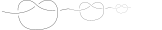
\includegraphics[scale=.7]{\figdir/countable-trefoil-arc.pdf}
    \caption{A very wild-looking tame arc}
  \end{figure}
  The trick is to define the $V_k$ to be a sequence of nested boxes as
  follows:
  \begin{figure}[H]
    \centering
    \includegraphics[scale=.7]{\figdir/countable-trefoil-arc-boxed.pdf}
  \end{figure}
  The reader should imagine these as properly nested rectangular
  prisms in $\RR^3$. For each of the $V_k$, define an ambient isotopy
  $F_k$ performing the following trick:
  \begin{figure}[H]
    \centering
    \includegraphics[scale=.7]{\figdir/countable-trefoil-arc-boxed-removing-1.pdf}
  \end{figure}
  \begin{figure}[H]
    \centering
    \includegraphics[scale=.7]{\figdir/countable-trefoil-arc-boxed-removing-2.pdf}
  \end{figure}
  \begin{figure}[H]
    \centering
    \includegraphics[scale=.7]{\figdir/countable-trefoil-arc-boxed-removing-3.pdf}
  \end{figure}
  \begin{figure}[H]
    \centering
    \includegraphics[scale=.7]{\figdir/countable-trefoil-arc-boxed-removing-35.pdf}
  \end{figure}
  \begin{figure}[H]
    \centering
    \includegraphics[scale=.7]{\figdir/countable-trefoil-arc-boxed-removing-4.pdf}
  \end{figure}
  \begin{figure}[H]
    \centering
    \includegraphics[scale=.7]{\figdir/countable-trefoil-arc-boxed-removing-5.pdf}
  \end{figure}
  \begin{figure}[H]
    \centering
    \includegraphics[scale=.7]{\figdir/countable-trefoil-arc-boxed-removing-6.pdf}
    \caption{An example $F_n$.}
  \end{figure}
  Observe that we can now apply
  \cref{thm:uniformly-convergent-ambient-isotopy} to show that the arc
  can be untangled in finite time. By contrast, we \emph{cannot} apply
  a similar argument to even a slightly-extended version of this arc:
  \begin{figure}[H]
    \centering
    \includegraphics[scale=.7]{\figdir/countable-trefoil-arc-extended.pdf}
    \caption[A non-example]{A case where we can't define the $V_n$
      such that $\lim_{n\to\infty} \mrm{diam}\pn{\bigcup_n V_n} \neq
      0$}
  \end{figure}
  % {\color{red} \LARGE WHY does this not cause problems for the lemmas
  % in chapter 5???????}
\end{example}
We have to be extremely careful when applying this argument, as it is
very easy to subtly fail the hypotheses without noticing. For
instance:
\begin{example}[Fox-Artin Curve]\label{ex:fox-artin-curve}
  Consider the following arc of \cite{FoxArtin}.
  \begin{figure}[H]
    \centering
    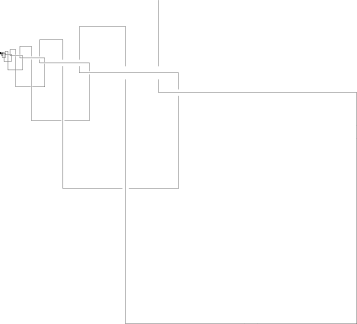
\includegraphics[scale=.2]{\figdir/loops-no-boxes.pdf}
    \caption{A non-example}
    \label{fig:loops-no-boxes}
  \end{figure}
  At first, it might appear reasonable to use
  \cref{thm:uniformly-convergent-ambient-isotopy} to ``undo'' each of
  the loops one-by-one. Certainly, one can define a sequence of boxes
  that satisfy both the \np{$\bigcup_{k=1}^\infty V_k$ is bounded in a
    compact set} and \np{$\lim_{n \to \infty} \bigcup_{n\in\NN} V_n =
    0$} conditions:
  \begin{figure}[H]
    \centering
    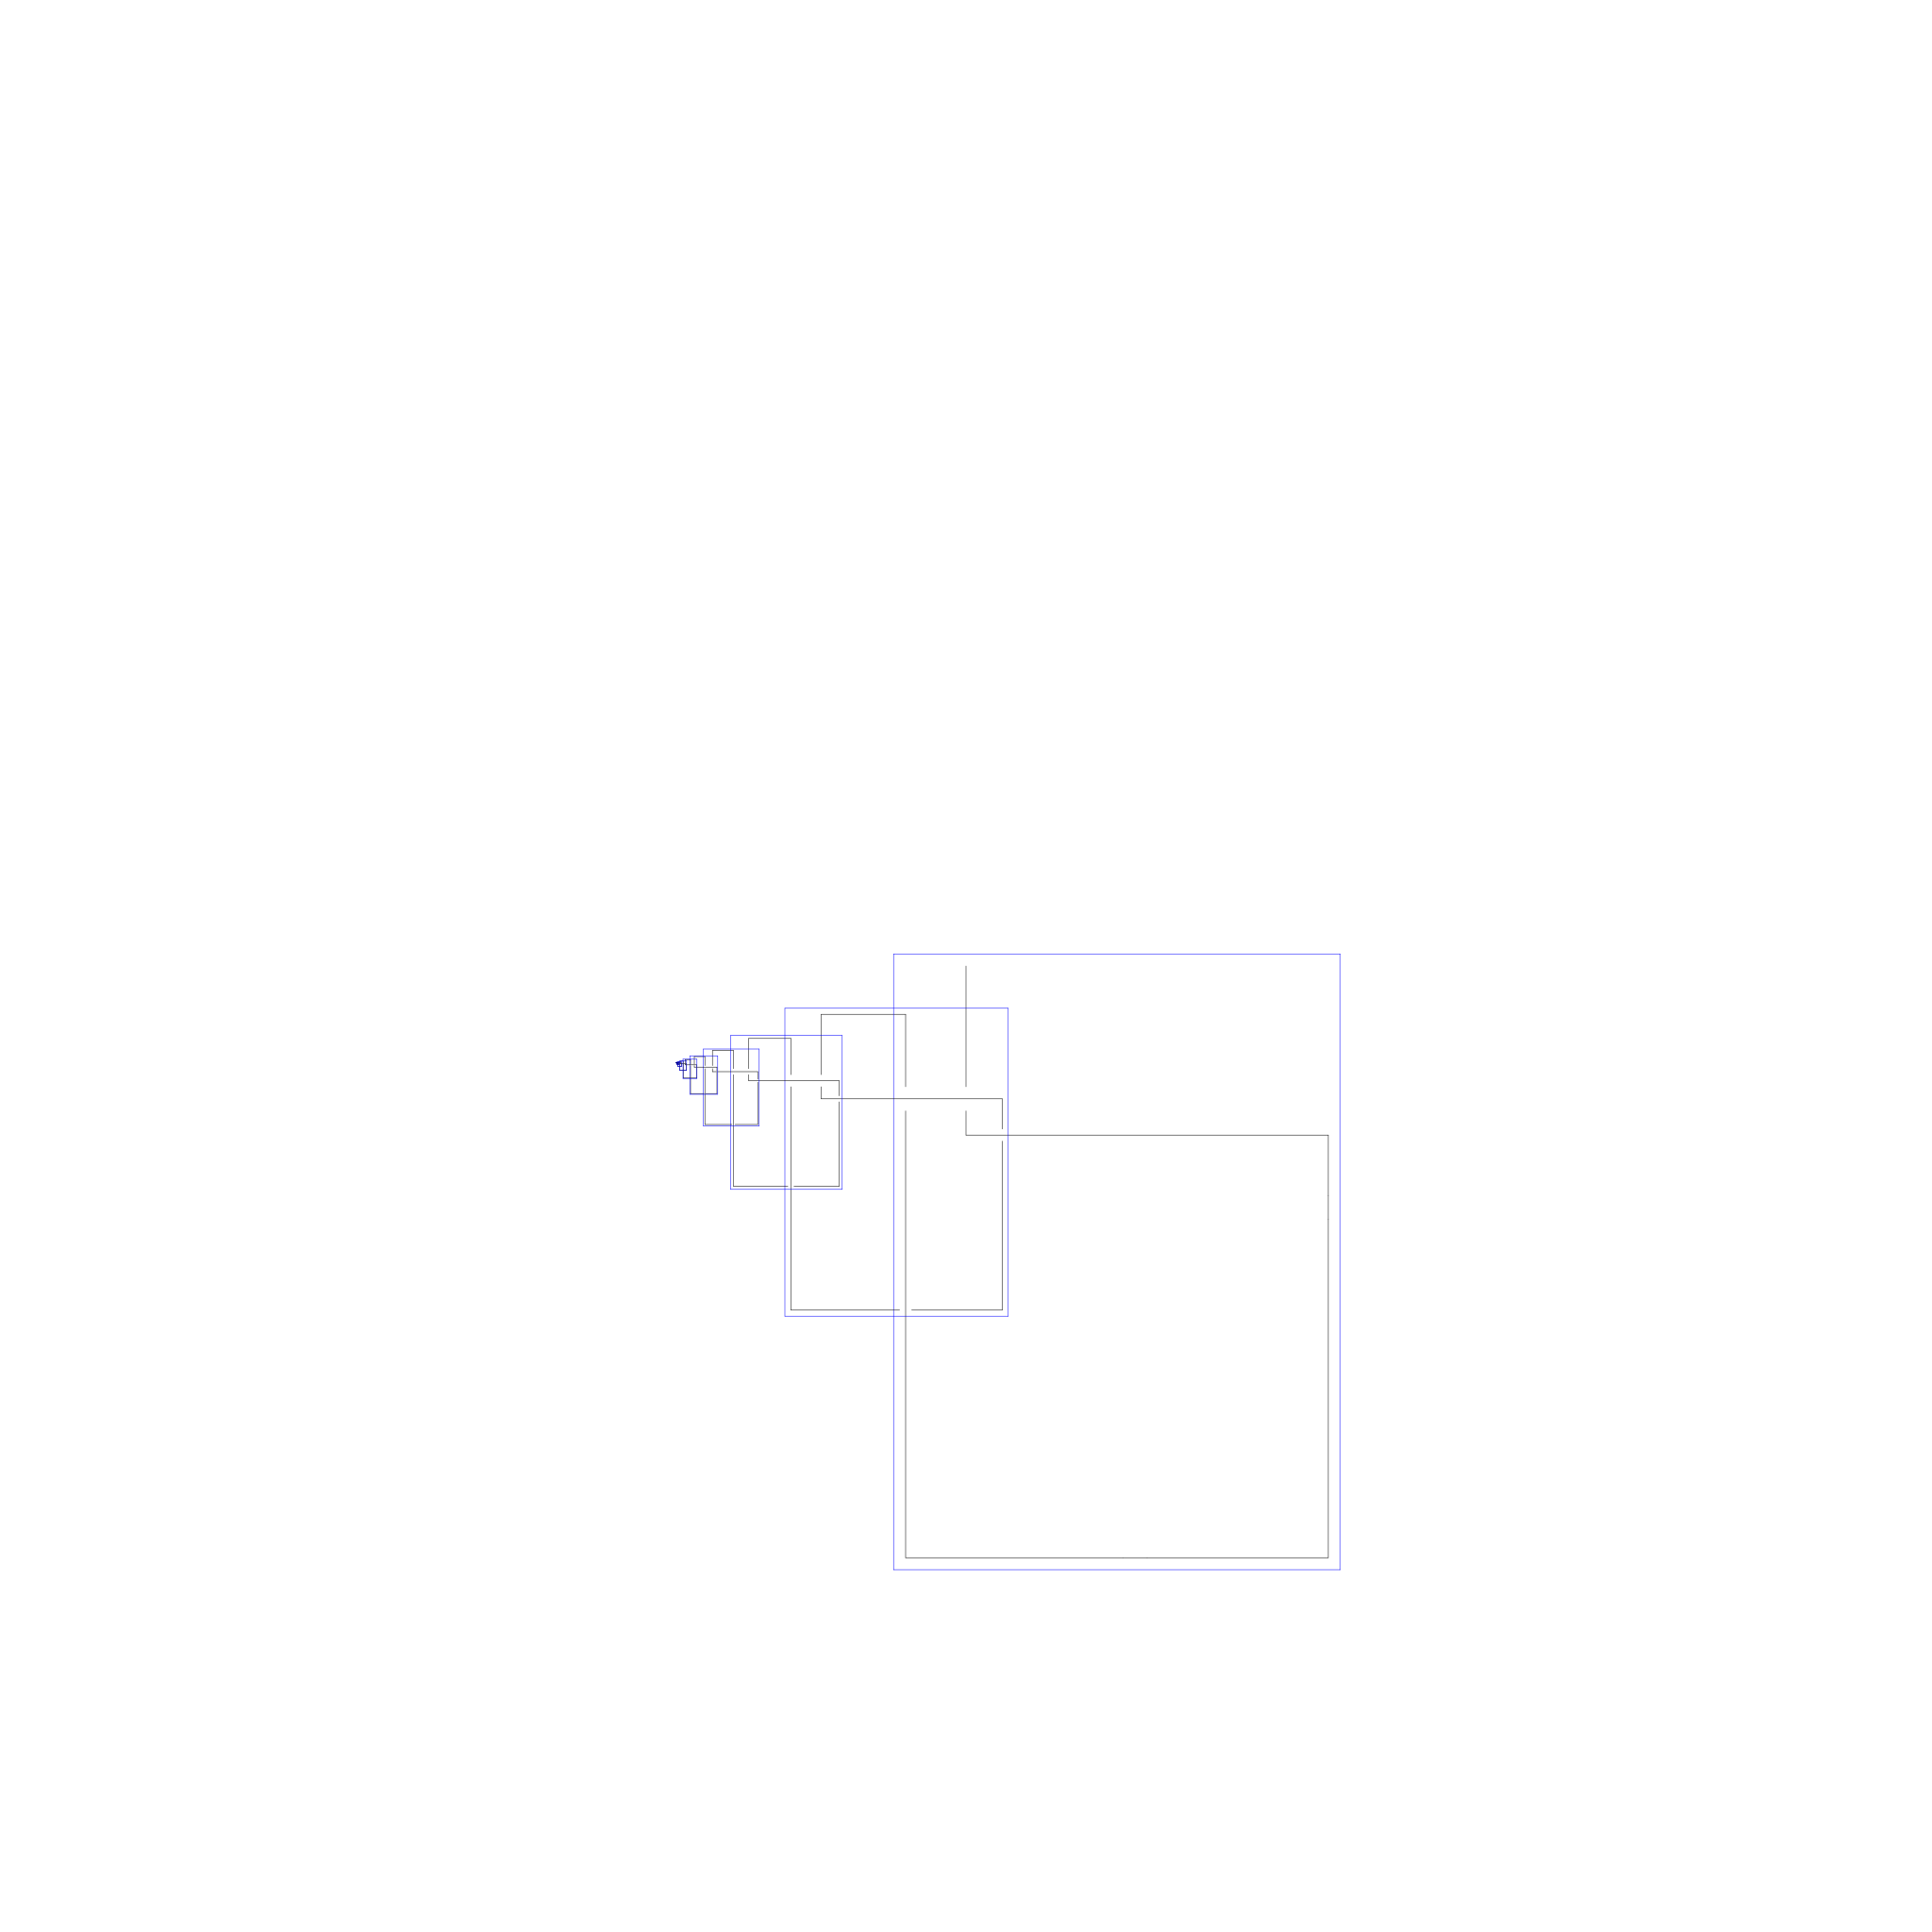
\includegraphics[scale=.2]{\figdir/loops-boxed.pdf}
    \caption{Some proposed $V_n$}
    \label{fig:loops-with-boxes}
  \end{figure}
  And indeed, one can find a sequence of ambient isotopies that take
  us arbitrarily close to the unknotted strand. Yet, we can
  \emph{prove} that this is actually a wild arc, using the invariant
  introduced by \cite{FoxArtin}.

  \begin{theorem}[Fox-Artin\footnote{Pronunciation Guide:
      \ipa{"a\textsubarch{5}ti:n}} Tameness
    Invariant] \label{thm:fox-artin-tameness}
    Suppose that $\gamma : [0,1] \into \RR^3$ is tamely embedded. Use
    $\ms S$ to denote the image
    \[
      \ms S = \fim{\gamma}{\bk{0,1}},
    \]
    and let $p = \gamma(0)$. Now, let $\set{V_n}_{n =1}^\infty$ be a
    properly-nested sequence of nested closed sets such that for each
    $n$, $p \in V_n^\circ$, and further
    \[
      \set{p} = \bigcap_{n=1}^\infty V_n.% } \subsetneq \cdots V_n
      % \subsetneq \cdots \subsetneq V_2 \subsetneq V_1.
    \]
    Then there exists $N \in \NN$ such that the homomorphism $i_*$
    \[
      \pi_1(V_N - \ms S) \xrightarrow{i_*} \pi_1(V_1 - \ms S)
    \]
    induced by $i : V_N - \ms S \into V_1 - \ms S$ is
    trivial.\footnote{For those who might not have seen it before:
      Here, $\pi_1$ denotes the fundamental group.}
  \end{theorem}
  We will try to be very thorough in the proof for those who might
  have seen the fundamental group before, but not had a lot of
  experience with it. This will likely strike others as a bit
  overkill. The version in Fox \& Artin's paper is much terser, and
  can be found on page 7.\footnote{In case the page numbering has
    gotten messed up, the paragraph begins with ``To show that $Y$ is
    wildly imbedded [sic] we first develop a necessary condition for
    an imbedding of an arc to be tame.''}
  \begin{proof}
    If $\gamma$ is tame, by definition, there exists a closed set $U
    \subseteq \RR^3$ and a homeomorphism $f : \RR^3 \to \RR^3$ such
    that we have
    \[
      (U, \ms S) \stackrel{\mathclap{f}}{\cong} (\text{3-ball},\
      \text{3-ball diameter}).
    \]
    Without loss of generality, we suppose that for all $n \in \NN$,
    $V_n \subseteq U$. Now, let $p' = f(p)$, $\ms S' = \fim{f}{\ms S}$
    (note this is the diameter), and let let $\pn{V_n'}_{n \in \NN}$
    be given by $V_n' = \fim{f}{V_n}$. Note that since $f$ is a
    homeomorphism, the $V_n'$ satisfy all the properties of the $V_n$.
    In particular, $p' \in {V'_1}^\circ$. Thus there exists
    $\varepsilon > 0$ such that
    \[
      B_\varepsilon(p') \subseteq V'_1.
    \]
    Also not that $\set{p'} = \bigcap_{n=1}^\infty V'_n$ implies that
    for some $N \in \NN$, we have
    \[
      V'_N \subseteq B_\varepsilon(p') \subseteq V'_1
    \]
    and thus
    \begin{equation}\label{eq:three-nested-subsets}
      \np{{V'}_N - \ms S'} \subseteq \np{B_\varepsilon(p') - \ms S'}
      \subseteq \np{{V'}_1  - \ms S'}.
    \end{equation}
    Choose some point $q \in W_N$ to serve as the base point for the
    fundamental groups of the sets in \cref{eq:three-nested-subsets}.
    Then observe that a
    \begin{enumerate}
      \item The inclusion $i : V'_N - S' \into V'_1 - S'$ is trivially
        given by composing $i_1 : V'_N - S' \into B_\varepsilon(p')$
        and $i_2 : B_\varepsilon(p') \into V'_1 - S'$
        \begin{figure}[H]
          \centering
          \begin{tikzpicture}
            \node (a) at (-1.5,0) {$V'_N - \ms S'$};
            \node (b) at (0,-1) {$B_\varepsilon(p')$};
            \node (c) at (1.5, 0) {$V'_1 - S'$};

            \draw[right hook->] (a) -- (c) node[midway, above] {$i$};
            \draw[right hook->] (a) -- (b) node[midway, below left] {$i_1$};
            \draw[right hook->] (b) -- (c) node[midway, below right] {$i_2$};
          \end{tikzpicture}
          \caption{Self-indulgent commutative diagram}
        \end{figure}
      \item $\pi_1(B_\varepsilon(p') - \ms S')$ is trivial (since
        $B_\varepsilon(p') - \ms S'$ is an open ball with a radius
        removed), and hence
      \item The induced map $i_{2,*} : \pi_1(B_\varepsilon(p') - \ms S')
        \into \pi_1(V_1' - \ms S')$ is trivial, and hence because $i_*
        = i_{2,*} \circ i_{1, *}$, $i_*$ is trivial.
        \begin{figure}[H]
          \centering
          \begin{tikzpicture}[scale=1.25]
            \node (a) at (-1.5,0) {$\pi_1(V'_N - \ms S')$};
            \node (b) at (0,-1) {$\pi_1(B_\varepsilon(p'))$};
            \node (c) at (1.5, 0) {$\pi_1(V'_1 - S')$};

            \draw[right hook->] (a) -- (c) node[midway, above] {$i_*$};
            \draw[right hook->] (a) -- (b) node[midway, below left]
            {$i_{*,1}$};
            \draw[right hook->] (b) -- (c) node[midway, below right]
            {$i_{*,2}$};
          \end{tikzpicture}
          \caption{Another self-indulgent commutative diagram}
        \end{figure}
    \end{enumerate}
    Now, since homeomorphism preserves the fundamental group, taking
    $V_N = \fpre{f}{V'_N}$ yields the desired result.
  \end{proof}
  One can verify that the $V_n$'s we drew in
  \cref{fig:loops-with-boxes} don't satisfy this property. What's
  the problem?

  The answer is that we lose bijectivity at $t = 1$ --- not on the
  curve itself, but rather on the ambient space. There's no way to
  undo the curve shown in \cref{fig:loops-with-boxes} without
  dragging infinitely-many points down into the wild point. To
  visualize why, imagine passing a solid torus vertically down
  through the first big loop.
  \begin{figure}[H]
    \centering
    \includegraphics[scale=.25]{\figdir/fox-artin-3d.pdf}
    \caption{A 3D perspective.}
    \label{fig:fox-artin-3d-torus}
  \end{figure}
  Observe that as we remove the first loop, we end up pulling the
  cylinder \emph{through} the second loop. Note, we're going to
  replace the torus with a line so as to make the diagrams easier to
  create. The same argument works either way; we felt the torus was
  more intuitive.
  \begin{figure}[H]
    \centering
    \includegraphics[scale=.25]{\figdir/fox-artin-3d-2.pdf}
    \caption{Pulling out a stitch.}
    \label{fig:fox-artin-pulling-out-a-stitch}
  \end{figure}
  As we iterate this process further, note that the string/torus will
  get dragged further and further downwards until finally converging
  to the wild point. In fact, the same result holds for a torus
  passing through \emph{any} such loop, so performing our proposed
  ambient isotopy would actually collapse infinitely-many points of
  the ambient space down to the wild point. Hence, this approach is no
  good, as it violates bijectivity.\footnote{An alternative argument
    is to show the ``undoing'' maps don't converge uniformly.}
\end{example}
\begin{note}
  While we explicitly drew the torus/line in the figures above, note
  that we're not actually thinking about embedding a torus into
  $\RR^3$. Rather, it's just a helpful visualization to see how the
  ambient space \emph{must} get bent as we perform our proposed
  sequence of ambient isotopies.
\end{note}
\begin{remark}
  One might wonder what would happen if instead we were allowed to
  move the loose end and pull \emph{it} through the stitches
  one-by-one. Note that doing so would require moving said strand
  arbitrarily close to the wild point; hence, it would be lost in the
  limit.
\end{remark}
The preceding two examples are meant to convey that we must proceed
with caution when dealing with
\cref{thm:uniformly-convergent-ambient-isotopy}.
\cref{ex:countable-trefoil-arc} shows that it's easy to take examples
that work and have slight extensions break them.
\cref{thm:uniformly-convergent-ambient-isotopy} shows us that it's
easy to be deceived by our pictures; we must be careful to be very
rigorous when entering the realm of general topological embeddings.

Now, we turn to our second tool: separating strands.

\section{Separating Strands}\label{sec:separating-strands}

\subsection{A Note on Notation in $S^1$}\label{sec:s1-notation}
From now on, we'll often have to work directly with sequences, open
sets, etc.\ in $S^1$. To that end we'll want to have some nice
notational shorthand to avoid having to say things like ``let $s_0,
s_1, s_3\in S^1$ such that, if thought of as an embedded $\RR^2$, we
would encounter $s_1$ before $s_2$ when traveling counterclockwise
around $S^1$ starting at $s_0$ \ldots'' Instead, we'll write this with
symbols.
\begin{itemize}
  \item By $s_0 \sprec s_1 \sprec \cdots \sprec s_n$, we mean that
    we'd encounter $s_0$ before $s_1$ before \ldots before $s_n$
    \emph{before} encountering $s_0$ a second time, if traversing
    around $S^1$ counterclockwise. Note, in displaystyle, $\sprec$
    looks like the following:
    \[
    s_0 \sprec s_1 \sprec \cdots \sprec s_n
    \]
    In analogy with $<$, $\leq$, the $\spreceq$ symbol allows the
    possibility of equality.
  \item By $\spn{s_0, s_1}$, $\sbk{s_0, s_1}$, we mean
    {\small
    \begin{align*}
      \spn{s_0, s_1} &= \set[Big]{s \in S^1 \MID s_0 \sprec s \sprec s_1}
      &
        \sbk{s_0, s_1} &= \set[Big]{s \in S^1 \MID s_0 \spreceq s \spreceq s_1}
    \end{align*}}
    and analogously for $\spb{s_0, s_1}$, $\sbp{s_0, s_1}$. We'll
    denote the topology generated by the $\spn{s_0, s_1}$ as $\tcirc$.
  \item Often, we'll think of $S^1$ as a metric space. We'll denote
    the ``ball of radius epsilon around $s$'' by
    $B_{\varepsilon}^\circlearrowleft(s)$.
  \item In general, we will try to refer to elements of $S^1$ by
    $s,t$, etc., but do note that $t$ is also used for the time
    variable in ambient isotopies.
\end{itemize}
Note, despite the notation above looking evocative of an orientation,
we are not actually thinking about $S^1$ as endowed with one. It just
so happens that in the below, we will often need to think about the
``next'' element of a sequence in $S^1$, but again this will be
detached from thinking of $S^1$ as oriented.









All of the theorems we show below work in $\RR^2$ as well as $\RR^3$,
which we can see by taking $K$ to be restricted to a 2D affine subset
of $\RR^3$.
\begin{proposition}\label{prop:separation}
  Let $K : S^1 \into \RR^3$ be an embedding, and let $I_0 = \sbk{s_0,
    t_0}$ and $I_1 = \sbk{s_1, t_1}$ be disjoint closed arcs of $S^1$.
  For the sake of notational compactness, define $Y_0 = \fim{K}{A_0}$
  and $Y_1 = \fim{K}{A_1}$. Then
  \[
    \inf_{\substack{p_0 \in Y_0 \\ p_1 \in Y_1}} d(p_1, p_2) > 0.
  \]
\end{proposition}
\begin{sproof}
  Since $K$ is an embedding, it is a homeomorphism onto its image.
  Now, since $I_0$, $I_1$ are disjoint compact sets, it follows that
  their images under $K$ are as well. Hence $Y_0, Y_1$ are disjoint
  compact sets. From this point, the claim can be proven by one of the
  following methods:
  \begin{enumerate}
    \item (With Analysis) Let $f : Y_0 \to \RR$ be defined as follows:
      for all $y_0 \in Y_0$, we have
      \[
      f(y_0) = \inf_{y_1 \in Y_1} d(y_0, y_1).
      \]
      Continuity of $f$ follows directly from the triangle inequality.
      Now, since $Y_0$, $Y_1$ are disjoiont, $f(y_0) > 0$ for all
      $y_0 \in Y_0$. Since $Y_0$ is compact, $f$ attains $\inf_{y_0
      \in Y_0} f(y_0)$ on $Y_0$, which yields the desired result.
    \item (With Topology) $\RR^3$ is Hausdorff; apply the fact that
      disjoint compact sets in a Hausdorff space can be separated by
      open sets. After a little finagling the proof should pop out.
      \qedhere
  \end{enumerate}
\end{sproof}
\begin{corollary}\label{cor:works-for-open}
  The same result holds if we replace ``disjoint closed arcs'' in
  \cref{prop:separation} with ``arbitrary sets that have disjoint
  closures.''
\end{corollary}
\begin{sproof}
  The exact same proof as above works. We just chose to state the
  specific case in \cref{prop:separation} first because it's more
  directly intuitive.
  % By ``separated'' we really mean the closures of the two arcs are
  % disjoint. Applying \cref{prop:separation} yields the desired result.
\end{sproof}

% The following proposition more or less states that if we take an
% \emph{arbitrary} collection of disjoint subarcs of $S^1$, then
% It's worth noting that even though we have this separation condition,
% we can still find
% \begin{proposition}\label{prop:inf-sep}
%   Let $K : S^1 \to \RR^3$ be a knot. Let $\set{A_i}_{i \in I}$ be a
%   collection of pairwise disjoint closed arcs of $S^1$, and define
%   $\set{X_i}_{i \in I}$ by $A'_i = K(A_i)$ for all $i \in I$. Finally,
%   let $i_0 \in I$ be arbitrary, and let
%   \[
%     X = \bigcup_{i \neq i_0} X_i.
%   \]
%   Then
%   \[
%     \abs{X_{i_0} \cap \ol{X'}} \leq 2,
%   \]
%   and if $A'_{i_0} \cap \ol{A'} = \varnothing$, then $d(A'_{i_0}, A')
%   > 0$.
% \end{proposition}
% \begin{proof}
%   First we prove $\abs{A_{i_0} \cap \ol{A}}\leq 2$. Observe that
%   because the $A_i$ are all disjoint, we have
%   \[
%     A \cap \bigcup_{i \neq i_0} A_i = 0
%   \]
%   which implies
%   \[
%     \bigcup_{i \neq i_0} A_i \subseteq A_{i_0}^c.
%   \]
%   It follows that
%   \[
%     \ol{\bigcup_{i \neq i_0} A_i} \subseteq \ol{A_{i_0}^c},
%   \]
%   hence $A_{i_0} \cap \ol{A} \subseteq A_{i_0} \cap \ol{A_{i_0}^c} =
%   \partial A_{i_0}$. Noting that $\abs{\partial A_{i_0}} = 2$, we get
%   the desired result.

%   It remains to show that if $A_{i_0} \cap \ol{A} = \varnothing$, then
%   $d(A_{i_0}, A) > 0$. First, note that $\ol{A}$ is closed, and
%   $\ol{A} \subseteq S^1$ implies $\ol{A}$ is bounded {\color{red} in
%     the metric induced by $\RR^n$?}. Now, observe that {\color{red}
%     $S^1$ inherits the Heine-Borel property from $\RR^n$}, so $\ol{A}$
%   is compact. By a similar proof to that of Proposition
%   \ref{prop:separation}, we get $d(A'_{i_0}, A') > 0$.
% \end{proof}
% \begin{remark}
%   (All variables are quantified as above). Note, there could exists
%   infinitely many distinct $i_0 \in I$ such that
%   \[
%     \abs{A'_{i_0} \cap \ol{A'}} \neq 0.
%   \]
%   In particular, consider the following partition of $[0,1]$: for all
%   $n \in \NN$, let $c_n = \frac{1}{n} - \frac{1}{n + 1}$. Then
%   consider the sets $A_{n,m}$ be given by for all $m \in \NN$,
%   \[
%     A_{n,m} = \bk{\frac{1}{n+1} + \frac{c_{n}}{2m + 1},\ \
%       \frac{1}{n+1} + \frac{c_{n}}{2m}}.
%   \]
%   Then if we take the $A_{n,m}$ together with sets of the form
%   \[
%     B_n = \bk{\frac{1}{n+1} + \frac{2}{3} c_n, \frac{1}{n}},
%   \]
%   and mod out by $0 \sim 1$, we see that for $n > 1$, each of the
%   $B_n$ satisfies $B_n \cap \ol{B'_n} = \frac{1}{n}$. We can visualize
%   this as follows:
%   \begin{figure}[H]
%     \centering
%     \includegraphics[scale=.7]{figures/infinite-gauss-sequence/countable-separation.pdf}
%     \caption{Visualization of the sets}
%     \label{fig:countable-sep}
%   \end{figure}
%   Note, we could apply a similar argument to show that we can actually
%   have infinitely many of the $B_n$ intersected on both sides.
% \end{remark}
% \begin{proposition}
%   Suppose that some arc contains
% \end{proposition}

The following theorem essentially says that we can separate strands in
a knot by closed, cone-shaped neighborhoods that only possibly
intersect at endpoints. Note, we'll index almost all variables with
$0$ subscripts to make it easier to refer to the analogues for the
other strand described at the end of the statement.
\begin{theorem}\label{thm:separating-strands}
  Let $K : S^1 \to \RR^3$ be a knot, and let $\sbk{s_0, t_0} \subseteq
  S^1$ with $s_0 \neq t_0$. Then there exists a nonempty, open,
  connected set $U_0 \subseteq \RR^3$ such that
  \begin{enumerate}
    \item $\fim{K}{\spn{s_0, t_0}} \subsetneq U_0$,
    \item $\fim{K}{\sbk{s_0, t_0}} \subseteq \ol{U_0}$, and
    \item $\fim{K}{\sbk{s_0, t_0}^c} \cap \ol{U_0} = \varnothing$.
  \end{enumerate}
  Further, given another disjoint arc $\sbk{s_1, t_1}$, the associated
  $U_1$ satisfies $\ol{U_0} \cap \ol{U_1} = \varnothing$.
\end{theorem}
\begin{proof}
  Use $I_0$ to denote $\sbk{s_0, t_0}$, and let its midpoint be
  denoted $m_0$. We first define a collection of ``nested'' subarcs of
  $I_0$ centered at $m_0$.\footnote{We put ``nested'' in scare quotes
    because we'll actually have uncountably many subarcs in this
    collection, so there's no canonical notion of ``successor'' or
    ``predecessor.''}

  Let $\ell$ be the length of $I_0$. Define $\varepsilon_{0, {\rm
      max}} = \frac{\ell}{2}$, and $E_0 \subseteq \RR$ by
  \[
    E_0 = \pn{0, \varepsilon_{0, \rm max}}.
  \]
  For all $\varepsilon_0 \in E$, let
  \[
    I_{\varepsilon_0} = \bcirc_{\varepsilon_0}(m_0),
  \]
  and observe that for all $\varepsilon_0' < \varepsilon_0$, we have
  \begin{equation}
    I_{\varepsilon_0'} \subsetneq I_{\varepsilon_0} \subsetneq
    I_0. \label{eq:containment}
  \end{equation}
  These are the desired ``nested'' subarcs of $I_0$.\footnote{For some
    intuition, note that as $\varepsilon_0 \incto \varepsilon_{0, \rm
      max}$, we have $I_{\varepsilon_0} \incto I_0$.} Also note that
  taking closures in \cref{eq:containment} preserves all of the
  containments.

  Now: Consider the complement $I_0^c$ in $S^1$, and note that it is
  an open arc of $S^1$. Also note that for all $\varepsilon_0 \in
  E_0$, $I_{\varepsilon} \subsetneq I_0$ implies
  \[
    \ol{I_{\varepsilon_0}} \cap \ol{I_0^c} = \varnothing,
  \]
  hence by \cref{cor:works-for-open}, $\delta_{\varepsilon_0}$ given
  by
  \[
    \delta_{\varepsilon_0} = d(\fim{K}{I_0^c},
    \fim{K}{I_{\varepsilon_0}})
  \]
  satisfies $\delta_{\varepsilon_0} > 0$. We use these
  $\delta_{\varepsilon_0}$'s to construct the desired open
  neighborhood $U_0$.

  For each $\varepsilon \in E$, let $U_{\varepsilon_0} \subseteq
  \RR^3$ be defined by
  \[
    U_{\varepsilon_0} = \set{\bm x \in \RR^3 \MID d(\bm x,
      \overrightarrow{K}(\ol{I_{\varepsilon_0}})) <
      \frac{\delta_{\varepsilon_0}}{3}}.
  \]
  Note that each of these $U_{\varepsilon_0}$ are open and
  nonempty.\footnote{We need the $\frac{1}{3}$ for the $\ol{U_0}\cap
    \ol{U_1} = \varnothing$ claim.} Also note that by definition of
  $\delta_{\varepsilon_0}$, for all $\varepsilon_0 \in E_0$, we have
  \[
    U_{\varepsilon_0} \cap I_0^c = \varnothing.
  \]
  Now, let
  \[
    U_0 = \bigcup_{\varepsilon_0 \in E_0} U_{\varepsilon_0}.
  \]
  Observe that $U_0$ is nonempty, open, and
  connected.\footnote{Connectedness follows from being a union of
    pairwise non-disjoint connected sets.} Also note that
  \begin{enumerate}
    \item $\fim{K}{\spn{s_0, t_0}} \subsetneq U_0$,
    \item $\fim{K}{\sbk{s_0, t_0}} \subsetneq \ol{U_0}$, and
    \item By the distributive property,
      \begin{align*}
        \fim{K}{I_0^c} \cap U_0
        &= \fim{K}{I_0^c} \cap \pn{\bigcup_{\varepsilon_0 \in E_0}
          U_{\varepsilon_0}} \\
        &= \bigcup_{\varepsilon_0 \in E_0} \pn{\fim{K}{I_0^c} \cap
          U_{\varepsilon_0}} \\
        &= \varnothing.
      \end{align*}
      Since $s_0, t_0 \not \in I_0^c$ it follows that $\fim{K}{I_0^c}
      \cap \ol{U_0}= \varnothing$ as well, as desired.
  \end{enumerate}
  This completes the proof of the claimed properties of $U_0$; it
  remains to show that given another arc $I_1 = \sbk{s_1, t_1}$ with
  $I_0 \cap I_1 = \varnothing$, the associated $U_1$ satisfies
  $\ol{U_0} \cap \ol{U_1} = \varnothing$.

  We proceed by contradiction. Suppose that $\ol{U_0} \cap \ol{U_1}
  \neq \varnothing$. We show that the points of intersection must be
  at the ends of the arcs $\fim{K}{I_0}$, $\fim{K}{I_1}$.

  To see this, note that by definition, for all $\varepsilon_0 \in
  E_0$,
  \[
    d(\fim{K}{I_{\varepsilon_0}},\ \fim{K}{I_1}) \geq
    \delta_{\varepsilon_0}.
  \]
  and similarly, for all $\varepsilon_1 \in E_1$,
  \[
    d(\fim{K}{I_{0}},\ \fim{K}{I_{\varepsilon_1}}) \geq
    \delta_{\varepsilon_1}.
  \]
  Because the $U_{\varepsilon_0}, U_{\varepsilon_1}$, were defined in
  in terms of $\frac{\delta_{\varepsilon_i}}{3}$, one can use a simple
  triangle inequality argument to show that for all $\varepsilon_0 \in
  E_0, \varepsilon_1 \in E_1$, we have
  \[
    d(U_{\varepsilon_0}, U_{\varepsilon_1}) > \frac{1}{3}
    \min\set{\delta_{\varepsilon_0}, \delta_{\varepsilon_1}}.
  \]
  It follows that if $d(U_0, U_1) = 0$, this must occur when one of
  the $\delta$'s is $0$ (i.e., $\varepsilon_0 = \varepsilon_{0, {\rm
      max}}$ or $\varepsilon_1 = \varepsilon_{1, {\rm max}}$, and
  hence $I_{\varepsilon_0} = I_0$, $I_{\varepsilon_1} = I_1$). This
  implies $\fim{K}{I_0}$, $\fim{K}{I_1}$ share an endpoint, a
  contradiction (\jiong) --- the arcs were assumed to be disjoint.
  \qedhere
\end{proof}
\begin{figure}[H]
  \centering
  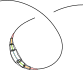
\includegraphics[scale=3]{figures/infinite-gauss-sequence/separation-cor-diagram-cropped.pdf}
  \caption{Example of $V$ and the $V_\varepsilon$}
  \label{fig:v-veps}
\end{figure}
We have a number of remarks to make about this theorem.
\begin{remark}
  Note that in general, as $\varepsilon_0 \incto \varepsilon_{0, \rm
    max}$, we get $\delta_{\varepsilon_0} \decto 0$. Further note that
  $\delta_{\varepsilon_0} : (0, \varepsilon_0) \to \RR$ (viewed as a
  function of $\varepsilon_0$) is continuous and can be continuously
  extended to a compact domain $[0, \varepsilon_{0, \rm max}]$ by
  taking $\delta_{\varepsilon_0}(0) = d\pn{m_0, \ol{A^c}}$ and
  $\delta_{\varepsilon_0}(\varepsilon_{0, \rm max}) = 0$. Hence
  $\delta_{\varepsilon_0}$ is in fact uniformly continuous.
  % It follows that even if $A$ is somewhat pathological (see
  % \cref{fig:everywhere-wild-3}, for instance), we can find a
  % double-sided-cone shaped envelope $U$ such that $A \subseteq U
  % \subseteq V$ such that the width of the cone increases linearly as
  % we go through $S^1$. {\color{red} is the wording here too vague?}
\end{remark}
\begin{remark}
  Note that because we chose to define the $I_{\varepsilon_0}$'s in
  terms of the $m_0$, if the parameterization of $K$ places $K(m_0)$
  closer to one of the endpoints $K(s_0)$ or $K(t_0)$, then we'll get
  a much thinner \& narrower $U_0$ than the one shown in
  \cref{fig:v-veps}. There are ways to change the proof above that
  avoid this issue, but we stuck with this version for simplicity.

  On a similar note, observe that the theorem makes no claims about
  \emph{substrands} of the strand $I_0$ being separated from each
  other. Indeed, $K$ could even be everywhere wild on $I_0$! The point
  is just that we can isolate the behavior of $K$ on $I_0$ from the
  behavior of $K$ on $S^1 \setminus I_0$, provided we keep our
  endpoints fixed.
\end{remark}
% \begin{remark}
%   On that note,
% \end{remark}
We have the following question:
\begin{question}
  Is the $U_0$ defined in \cref{thm:separating-strands} always
  homeomorphic to $\RR^3$?
\end{question}
If we restrict ourselves to the analogous theorem for $\RR^2$, a
``yes'' follows from the \cref{thm:jordan-schoenflies}
(Jordan-Schoenflies; see next section). In $\RR^3$, we don't have such
a result; in particular, we can find pathological objects like the
\emph{Alexander horned sphere} that don't partition our space nicely
into two topological $3$-balls. Is it possible to find a knot for
which the $U_0$ displays this kind of behavior? If not, this would
provide us a nice correspondence with \emph{local flatness}.


% Either way, the $\RR^2$ version gets us a very important theorem. One
% should note that we are \emph{not} guaranteed an analogous theorem in
% $\RR^3$.
% \begin{theorem}\label{thm:countable-convexity}
%   Let $K : S^1 \into \RR^2$ be an embedding, and let $\sbk{s_0, t_0}
%   \subseteq S^1$. Let $U_0$ be the neighborhood guaranteed by
%   \cref{thm:separating-strands}. Then $U_0$ can be written as a
%   countable union of convex sets.
% \end{theorem}
% \begin{sproof}[Sketch]
%   By \cite{Kojman1990Oct}, it suffices to show that neither of the
%   following hold:
%   \begin{enumerate}
%     \item There is a perfect subset\footnote{Recall, a set is perfect
%       if it is closed and has no limit points.} $A \subseteq U_0$ such
%       that for every pair of distinct points $a_0, a_1 \in A$, the
%       convex hull $\ip{a_0, a_1} \not\subseteq A$, or
%     \item There is no such set $A$ as defined above, but there
%       \emph{does} exist a perfect set $B \subseteq U_0$ such that for
%       all distinct $b_0, b_1$, $\ip{b_0, b_1} \subseteq B$, \emph{but}
%       adding a third distinct point $b_2 \in B$ yields $\ip{b_0, b_1,
%       b_2} \not\subseteq U_0$.
%   \end{enumerate}
%   We proceed as follows. Note that $(U_0, \fim{K}{\sbk{s_0, t_0}})
%   \cong (\mbb{D}^2, \text{diameter of $\mbb{D}^2$})$.kkkkkkkkkkkkkkkk
% \end{sproof}


% We have the following conjecture:
% \begin{conjecture}
%   The $U_0$ defined in \cref{thm:separating-strands} is homeomorphic
%   to $\RR^3$.
% \end{conjecture}
% It seems this follows fairly easily from \cref{thm:jordan-schoenflies}
% (Jordan-Schoenflies) in $\RR^2$. In $\RR^3$, the situation is a bit
% less clear, since we


% straightforward in $\RR^2$. In $\RR^3$,
% The importance of this result comes from the following:
% \begin{proposition}
%   Quantify all variables as in \cref{thm:separating-strands} above.
%   Then in $\RR^2$, $U_0$ is homeomorphic to $\RR^2$.
% \end{proposition}
% \begin{sproof}
%   Follows from \cref{thm:jordan-schoenflies}
% \end{sproof}

%%% Local Variables:
%%% TeX-master: "../../kobayashi-thesis"
%%% End:
